\section{Experimental Results}
In this section, the three proposed algorithms for $l1$-norm minimization problem will be applied to our \emph{Athemium dataset} retrieved from a monitoring system presented in the next section. The performance of these algorithms will then be compared with the edge detection one~\cite{Hart92} to evaluate the improvement. Besides, they are also applied to detect the state of devices in the Reference Energy Disaggregation Dataset (REDD)~\cite{Kolter11redd}, one of the biggest publicly available dataset for NILM research community. In REDD, the power consumption in two main phases of electricity in six households in the USA is measured every second during many days and the power consumption of some typical devices is retrieved every 3-4 seconds.




\subsection{Athemium data collection}

\begin{figure}[h]
\centering
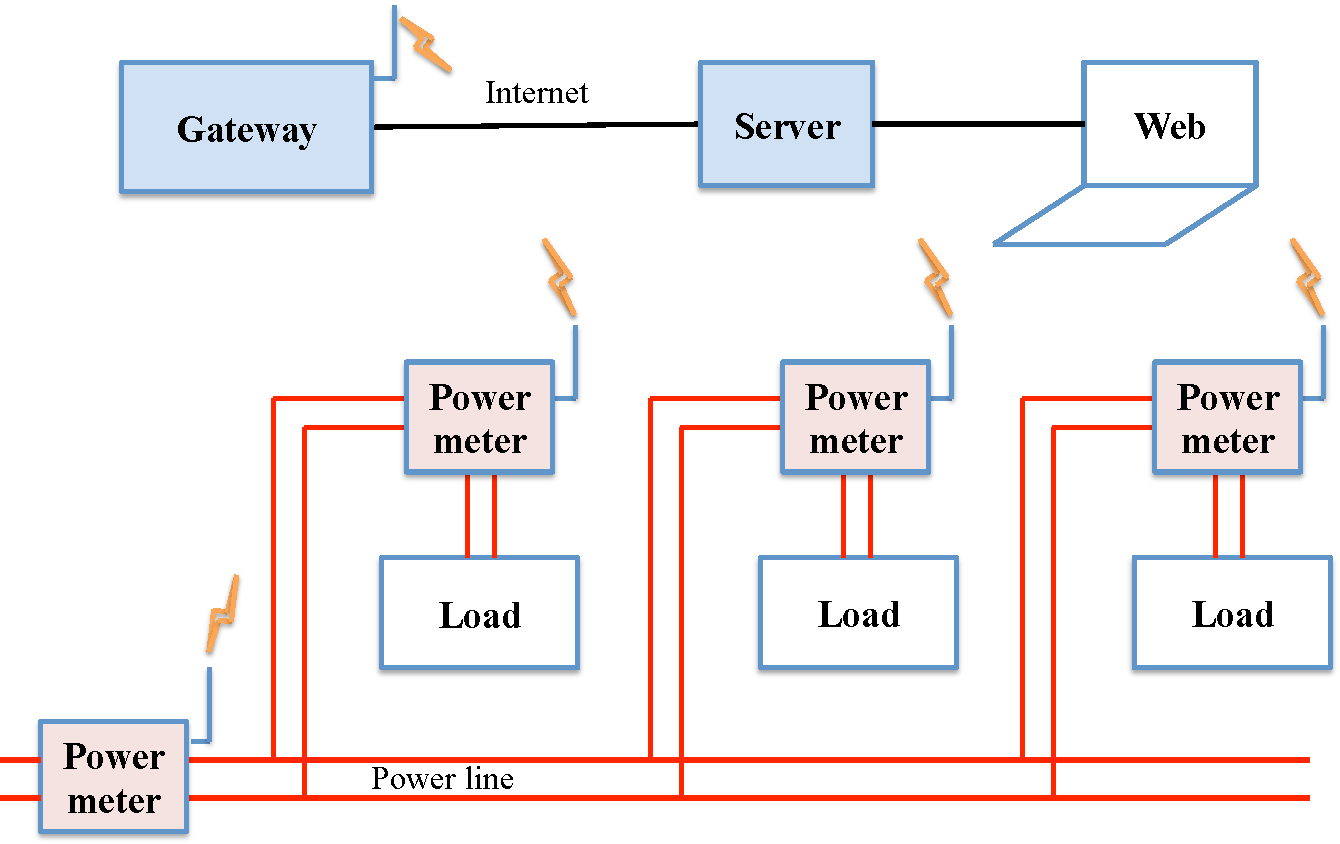
\includegraphics[width=.8\textwidth]{./chapters/chapter3/images/measurement_system.pdf} 
\caption{Smart meters network to retrieve the Athemium data.} 
\label{fig:L2} 
\end{figure}

To retrieve the Athemium data, a meter network supporting Zigbee wireless communications provided by Athemium company~\cite{Athemium} is deployed in the coffee room of our laboratory. 
The smart meter network is illustrated in Figure~\ref{fig:L2}, in which each device is attached to an individual meter. Data provided by these meters are used to learn the characteristics of each device as well as considered as ground truth data to evaluate performance of disaggregation algorithms. Additionally, a global power meter is also installed at the main circuit to measure the aggregate power consumption, which will be used to detect the operating states of each device. These power meters, fabricated by Netvox Technology Company~\cite{Netvok}, support wireless communication to send the power measurement to a gateway, which will forward it to an Athemium server through Internet connection. A web interface allows users to observe and download data. This interface lists all deployed power meters and sensors as well as their detailed parameters such as name, position, label, MAC address, as illustrated in Figure~\ref{fig:L22}. Besides, users can also display the power consumption of each device during hours, days, weeks, months and years.
\begin{figure}[htb]
\begin{minipage}[h]{1\linewidth}
\centering
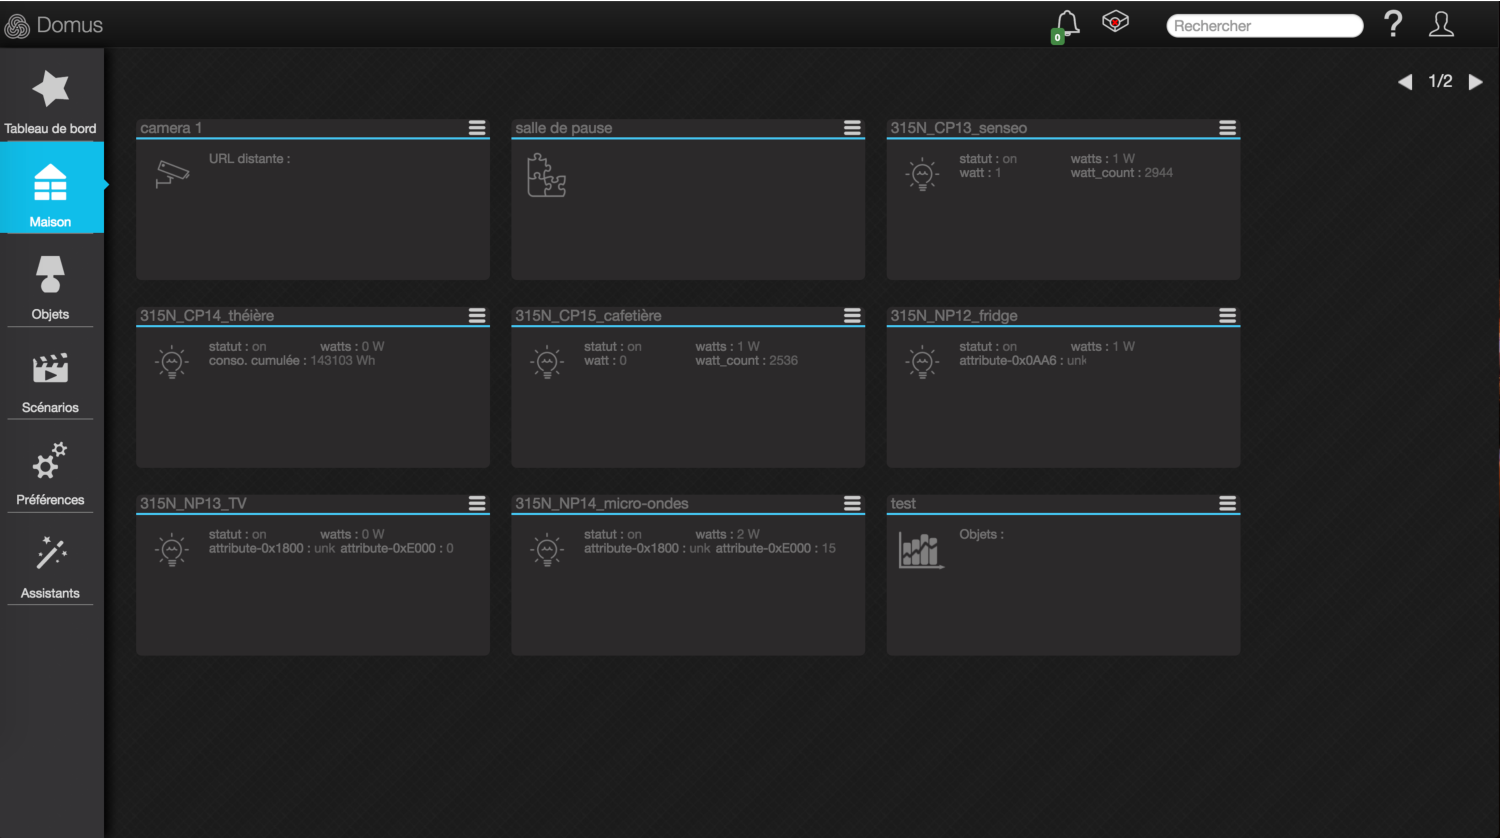
\includegraphics[width=0.8\textwidth]{./chapters/chapter3/images/A_web1.pdf}
%  \vspace{1.5cm}
\centerline{(a) List of deployed meters and sensors}\medskip
\end{minipage}
\hfill
\begin{minipage}[h]{0.48\linewidth}
\centering
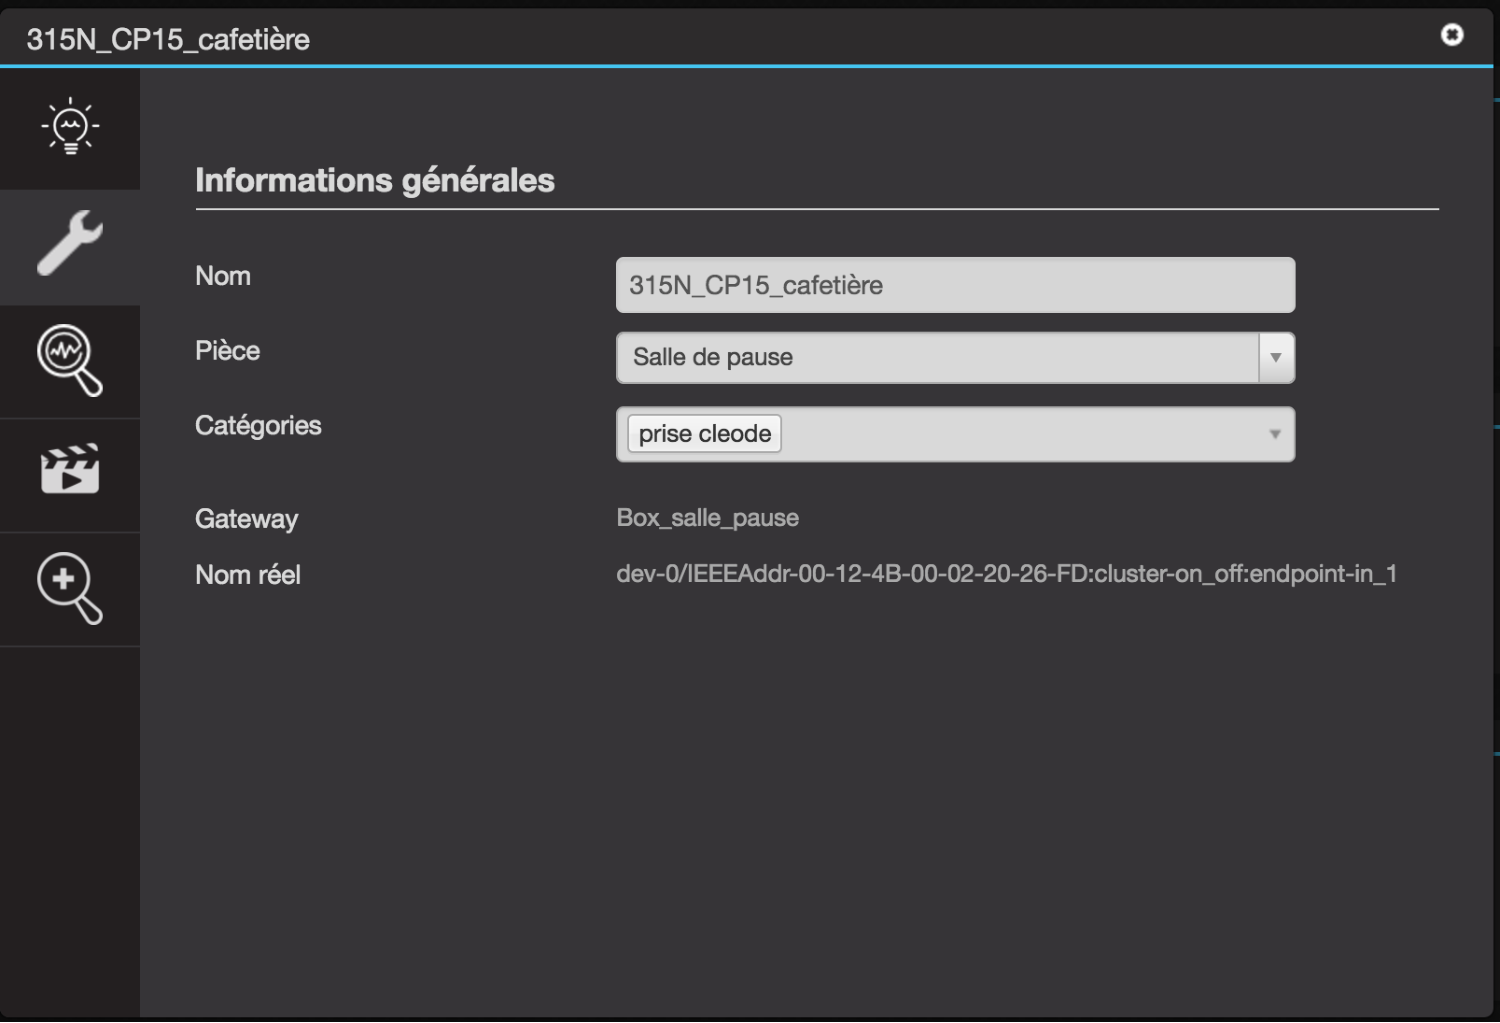
\includegraphics[width=1\textwidth]{./chapters/chapter3/images/A_web2.pdf}
%  \vspace{1.5cm}
\centerline{(b) Meters configuration}\medskip
\end{minipage}
\hfill
\begin{minipage}[h]{0.48\linewidth}
\centering
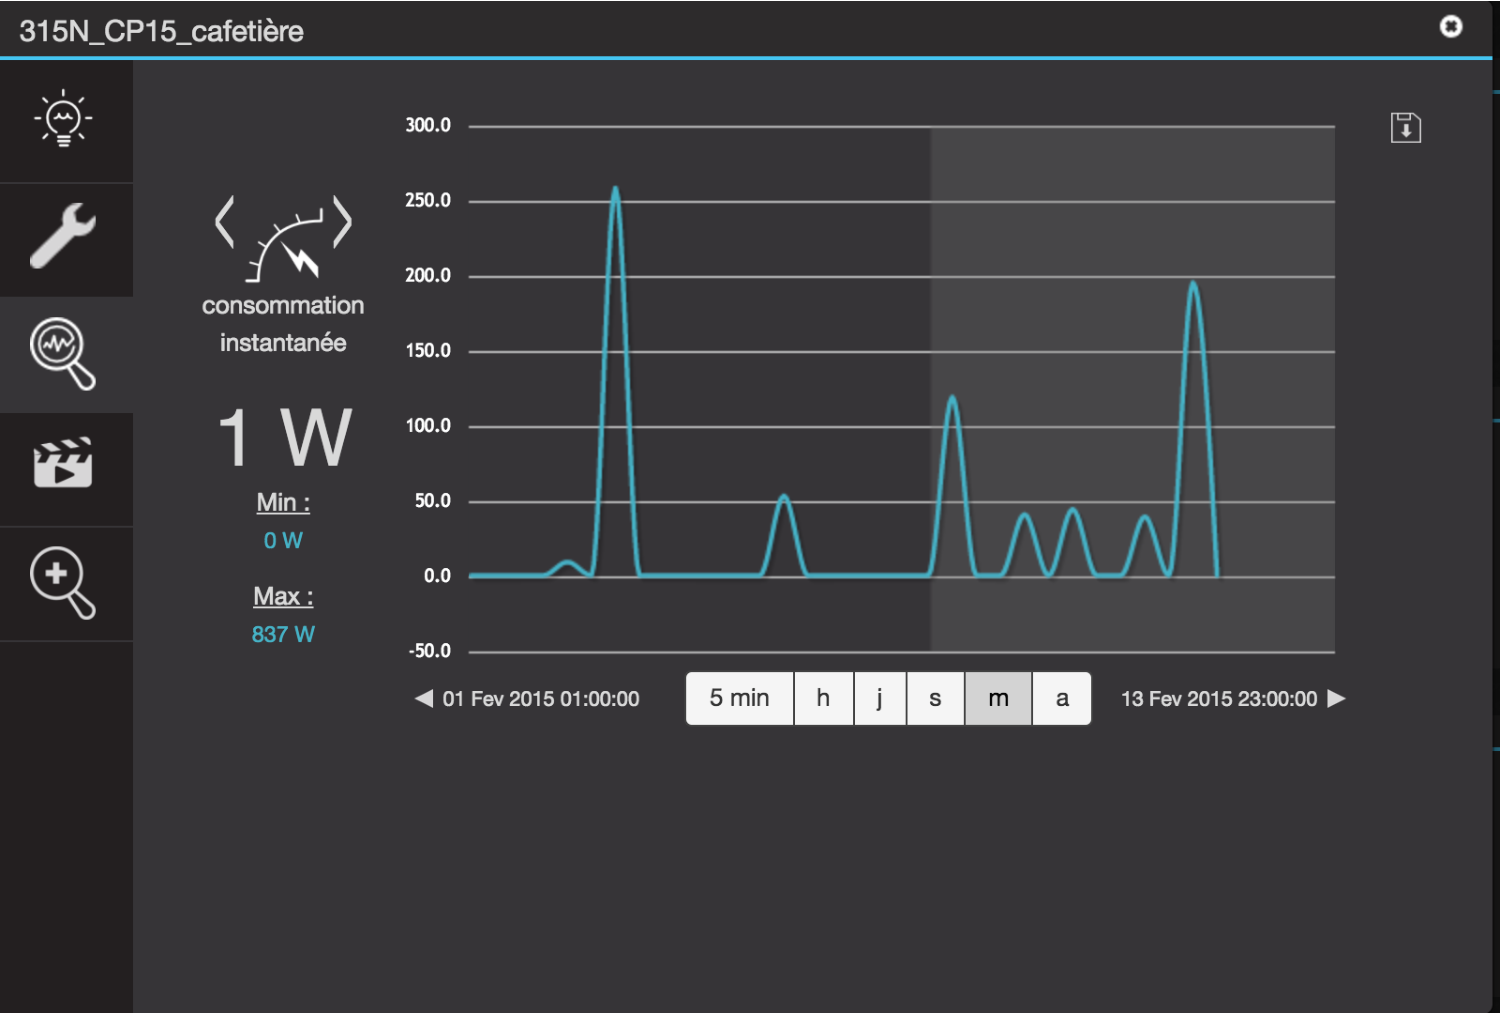
\includegraphics[width=1\textwidth]{./chapters/chapter3/images/A_web3.pdf}
%  \vspace{1.5}
\centerline{(c) Power measurement display}\medskip
\end{minipage}
\caption{Athemium web interface.}
\label{fig:L22}
%
\end{figure}

In this experiment, six devices including fridge, coffee machine, kettle, microwave, television and screen monitor are connected to power meters, as shown in Figure~\ref{fig:L23}. Other loads such as lamps, telephone chargers, Internet modem, outlets, etc., are considered as noise sources. Table~\ref{table:t1} shows the power demand of each device, while an example of their daily power consumption as well as aggregate power is illustrated in Figure~\ref{fig:L3}. Based on these retrieved data, state transition probability of each device can be calculated as presented in Figure~\ref{fig:L1}.

\begin{figure}
\centering
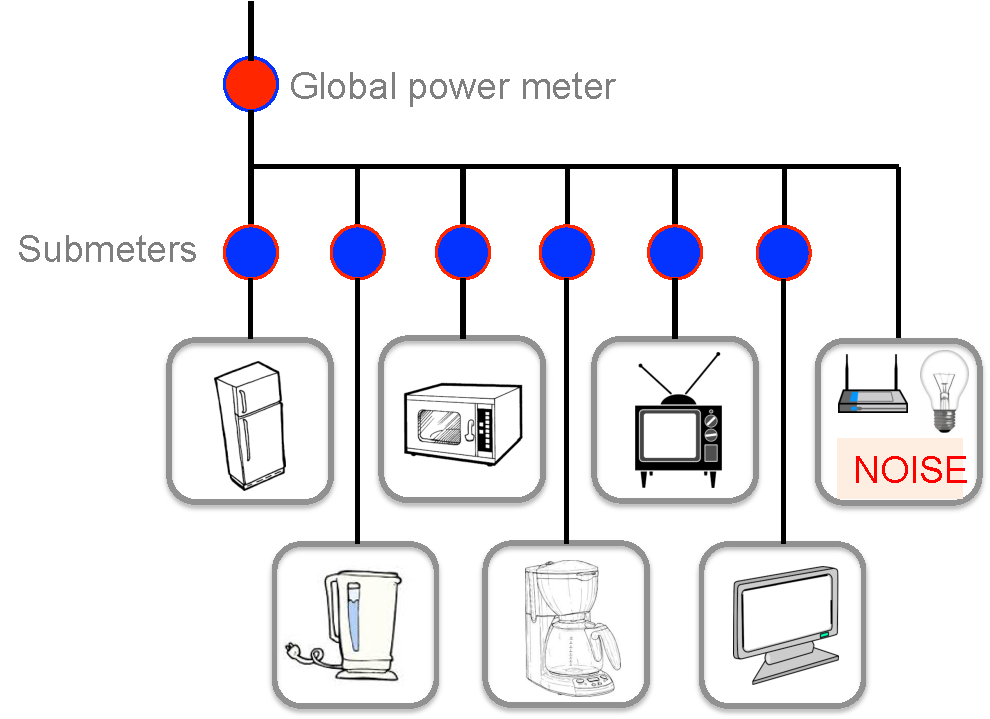
\includegraphics[width=.65\textwidth]{./chapters/chapter3/images/A_topo.pdf} 
\caption{Athemium power measurement: a global power meter measures the aggregate power consumption and some sub-meters provide training data and ground truth data of each device.} 
\label{fig:L23} 
\end{figure}

\begin{table}
\caption{Power demand of devices in Athemium dataset.}\label{table:t1}
\begin{center}
\begin{tabular}{|c|c|c|c|}
\hline
Power demand (Watt)& State 1&State 2&State 3 \\ \hhline{|=|=|=|=|}
Fridge &75& & \\ \hline
Coffee machine &823 &797 & 214 \\ \hline
Kettle & 1667 & 1692 & 1635\\ \hline
Microwave &1350 & 1316 & 1290 \\ \hline
Television & 203 & 29 & \\ \hline 
Screen monitor & 727 & & \\ \hline
\end{tabular}
\end{center}
\end{table}



\begin{figure}
\begin{minipage}[b]{1.0\linewidth}
  \centering
  \centerline{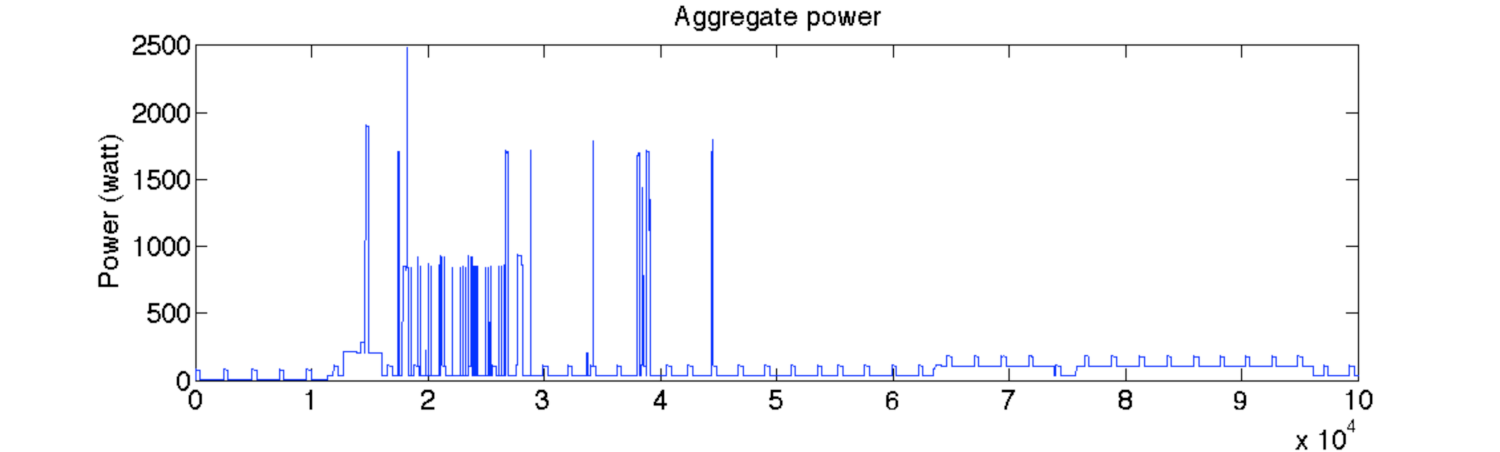
\includegraphics[width=1\textwidth]{./chapters/chapter3/images/A_aggpow.pdf}}
%  \vspace{2.0cm}
  \centerline{(a) Aggregate power consumption}\medskip
\end{minipage}
\begin{minipage}[b]{1.0\linewidth}
  \centering
  \centerline{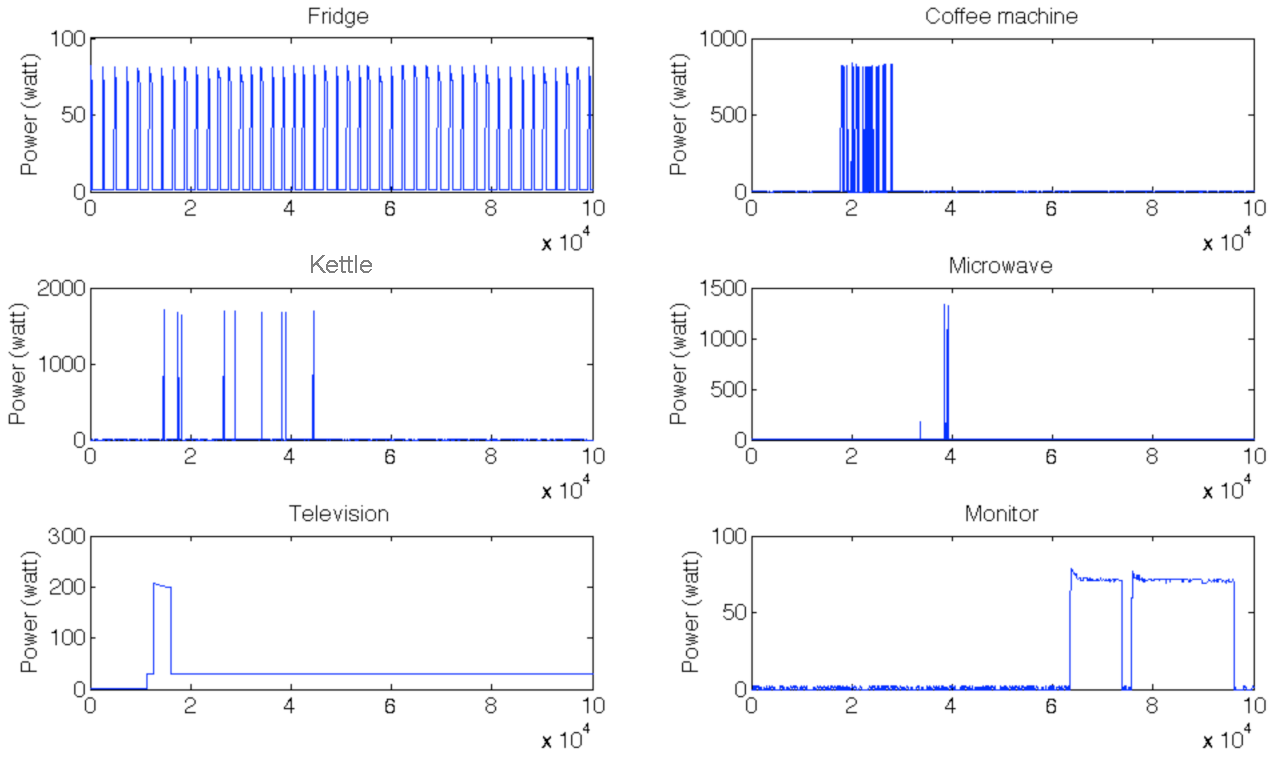
\includegraphics[width=1\textwidth]{./chapters/chapter3/images/A_pow.pdf}}
%  \vspace{2.0cm}
  \centerline{(b) Power consumption of each individual device}\medskip
\end{minipage}
\caption{Power measurement of the devices in Athemium dataset during one day.}
\label{fig:L3} 
\end{figure}




\subsection{Results and Evaluation}\label{resultl1}
To evaluate the algorithms, three metrics are used including \textit{precision} ($pr$), \textit{recall} ($rc$) and \textit{F-measure} ($Fm$)~\cite{Olson2008}, which are theoretically defined as:
\begin{eqnarray}\label{eva-metrics}
pr &=& \frac{TP}{TP+FP},\\
rc &=& \frac{TP}{TP+FN},\\
Fm &=& \frac{2\times pr \times rc}{pr+rc},
\end{eqnarray}
where $TP$, $FP$ and $FN$ are the number of true positives, false positives and false negatives, respectively. A true positive is a true detection of an event, while a false positive (false negative) means a non-event (event) being not correctly detected. As a consequence, the precision can be considered as the reliability of a detected event and the recall is the sensibility to the events of algorithms. Meanwhile, F-measure is interpreted as a weighted average of the precision and recall, which reaches its best value at 1 and worst at 0. For example, if there are 1500 of 2000 time instants that a fridge operates are correctly detected, we have $TP=1500$ and $FN=500$. Similarly, $FP = 200$ if 200 instants that the device is turned off are detected as on. As a consequence, we can obtain:

\begin{eqnarray*}
pr &=& \frac{1500}{1500+200} = 0.88,\\
rc &=& \frac{1500}{1500+500} = 0.75,\\
Fm &=& \frac{2\times 0.88 \times 0.75}{0.88+0.75} = 0.81.
\end{eqnarray*}


\begin{figure}
\centering
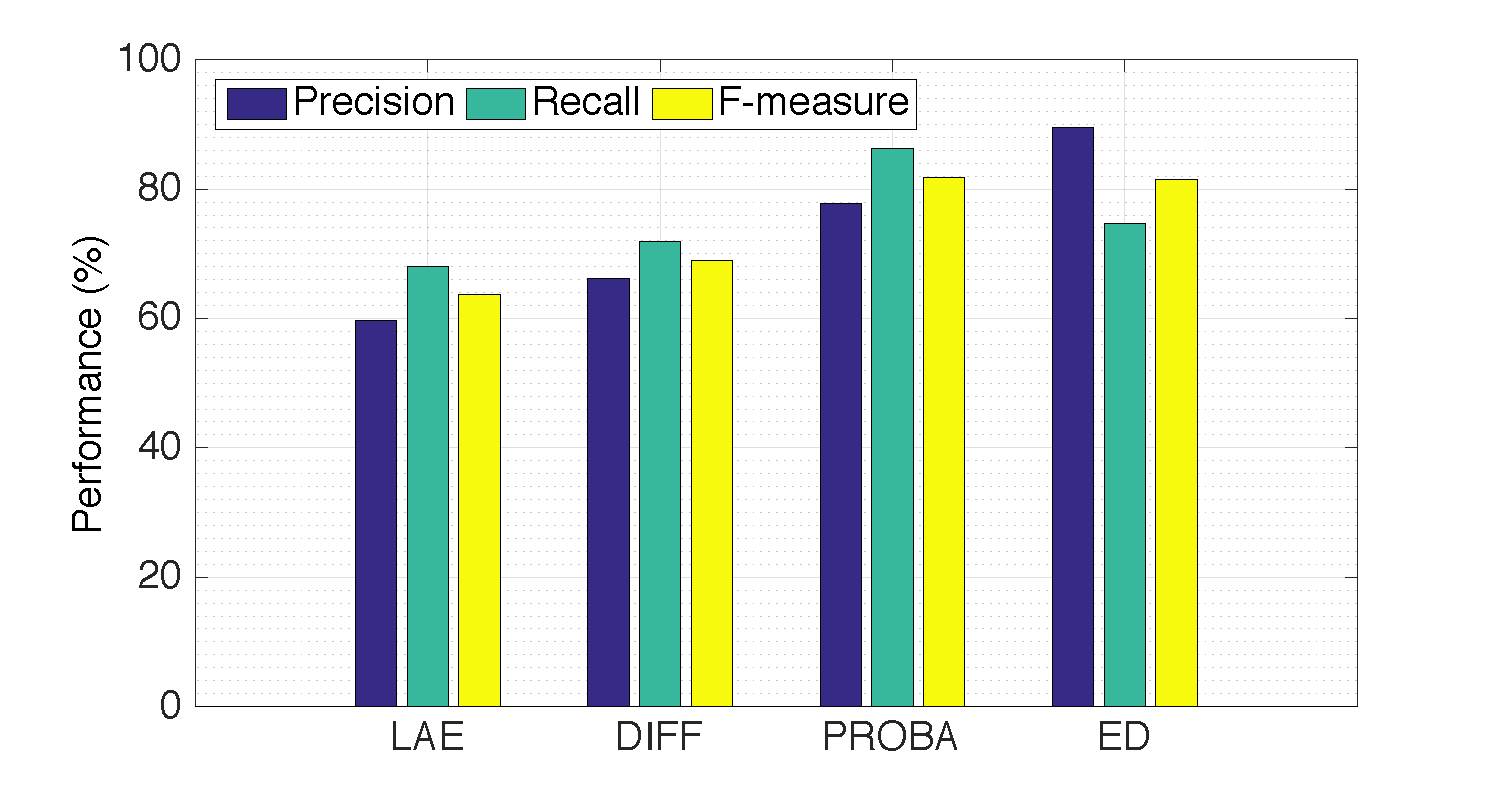
\includegraphics[width=.8\textwidth]{./chapters/chapter3/images/l1_perf.pdf} 
\caption{Performance of the proposed algorithms including LAE, state difference based (DIFF) and transition probability based (PROBA) compared with edge detection algorithm (ED) applied to Athemium data.}
\label{fig:L4} 
\end{figure}
In our Matlab simulation, 30$\%$ of data are used to learn the parameters while state detection algorithms are applied to the remaining.
In Figure~\ref{fig:L4}, performance of the three proposed algorithms with Athemium dataset is shown in comparison with the edge detection algorithm. Apparently, the brute force algorithm without any additional information shows a worse performance than the edge detection approach. While the edge detection algorithm can detect the devices with an overall precision of 89.58$\%$ and recall of 74.65$\%$, the LAE based algorithm only shows a poor performance of 60$\%$ and 69$\%$, respectively. This result comes from the fact that there are some devices consuming a close power level, e.g. coffee machine (214W) and television (203W). Nevertheless, because the coffee machine has three states, the detection based on the edges height is more effective. This is also the reason why considering the state transition of the devices, executed by selecting a subset of suitable combinations giving an error closed to the least value and applying the difference between each combination with the previous state as a criterion to select the solution, can increase the performance of the brute force algorithm. Concretely, the precision can be improved from 60$\%$ to 67$\%$ and the recall from 69$\%$ to 71$\%$. Especially, the performance improvement is more significant if the state transition probability is applied instead of the Hamming distance between the state combinations. Although performing a lower precision (79$\%$ \emph{vs.} 89.58$\%$), the probability based algorithm shows a better recall (87$\%$) than the edge detection one (74.65$\%$), which results in a close F-measure (81.8$\%$ \emph{vs.} 81.43$\%$) for both algorithms.

Table~\ref{table:t2} details the performance of the proposed algorithms correlated to each individual device. Apparently, the LAE based algorithm shows a high reliability in detecting the kettle ($pr=96.89\%$) while it is sensible to the operation of the coffee machine ($rc=99.05\%$) and television ($rc=95.74\%$). The fridge and microwave with many spikes on the power signal are identified with a lower precision than other devices ($pr=43.08\%$ and $pr=44.30\%$, respectively). Meanwhile, the state difference based algorithm allows to significantly improve the performance of the television (F-measure from 86.12$\%$ to 91.02$\%$) and kettle (60.53$\%$ to 76.9$\%$). With the transition probability based algorithm, the remarkable increase of the performance corresponds to the fridge (56.22$\%$ to 75.30$\%$), kettle (60.53$\%$ to 84.43$\%$), microwave (56.03$\%$ to 67.53$\%$) and monitor (55.25$\%$ to 79.13$\%$).

\begin{table}
\caption{Detailed performance of the three proposed algorithms including LAE based, state difference based (DIFF) and state transition probability based (PROBA) to detect each device: fridge (FR), coffee machine (CF), kettle (TE), microwave (MW), television (TV) and monitor (MO).}\label{table:t2}
\begin{center}
\begin{tabular}{|c|c|c|c|c|c|c|c|c|c|}
\hline
&\multicolumn{3}{|c|}{Precision ($\%$)} & \multicolumn{3}{|c|}{Recall ($\%$)}&\multicolumn{3}{|c|}{F-measure ($\%$)}\\
\hline
&LAE & DIFF & PROBA & LAE & DIFF & PROBA & LAE & DIFF & PROBA\\
\hline
FR & 43.08 &44.24&63.80&80.88&73.95&91.86&56.22&55.36&75.30\\
\hline
CM&76.64&80.25&76.34&99.05&98.94&98.90&86.42&86.62&86.17\\
\hline
TE &96.89&98.97&98.98&44.01&62.88&73.61&60.53&76.90&84.43\\
\hline
MW & 44.30 & 47.01&57.63&76.22&81.55&81.55&56.03&59.64&67.53\\
\hline
TV &78.25&86.99&83.05&95.74&95.44&95.79&86.12&91.02&89.97\\
\hline
MO & 55.52&57.80&89.83 &54.99&59.86&70.71&55.25&56.67&79.13\\
\hline
\end{tabular}
\end{center}
\end{table}

As mentioned in the previous section, an important parameter affecting the performance of the state difference based and state transition probability based algorithms for $l1$-norm minimization problem is the threshold $\gamma$ to select the retained combinations. If this threshold is too small, the true combination may be left out. In contrast, if it is too high, too many combinations are maintained and that may cause the decrease of the performance as well as the increase of the execution time. Figure~\ref{fig:L6} shows the effect of the threshold $\gamma$ on the performance of the algorithm based on the state transition probability with the best result obtainable at $\gamma = 3$.

\begin{figure}
\centering
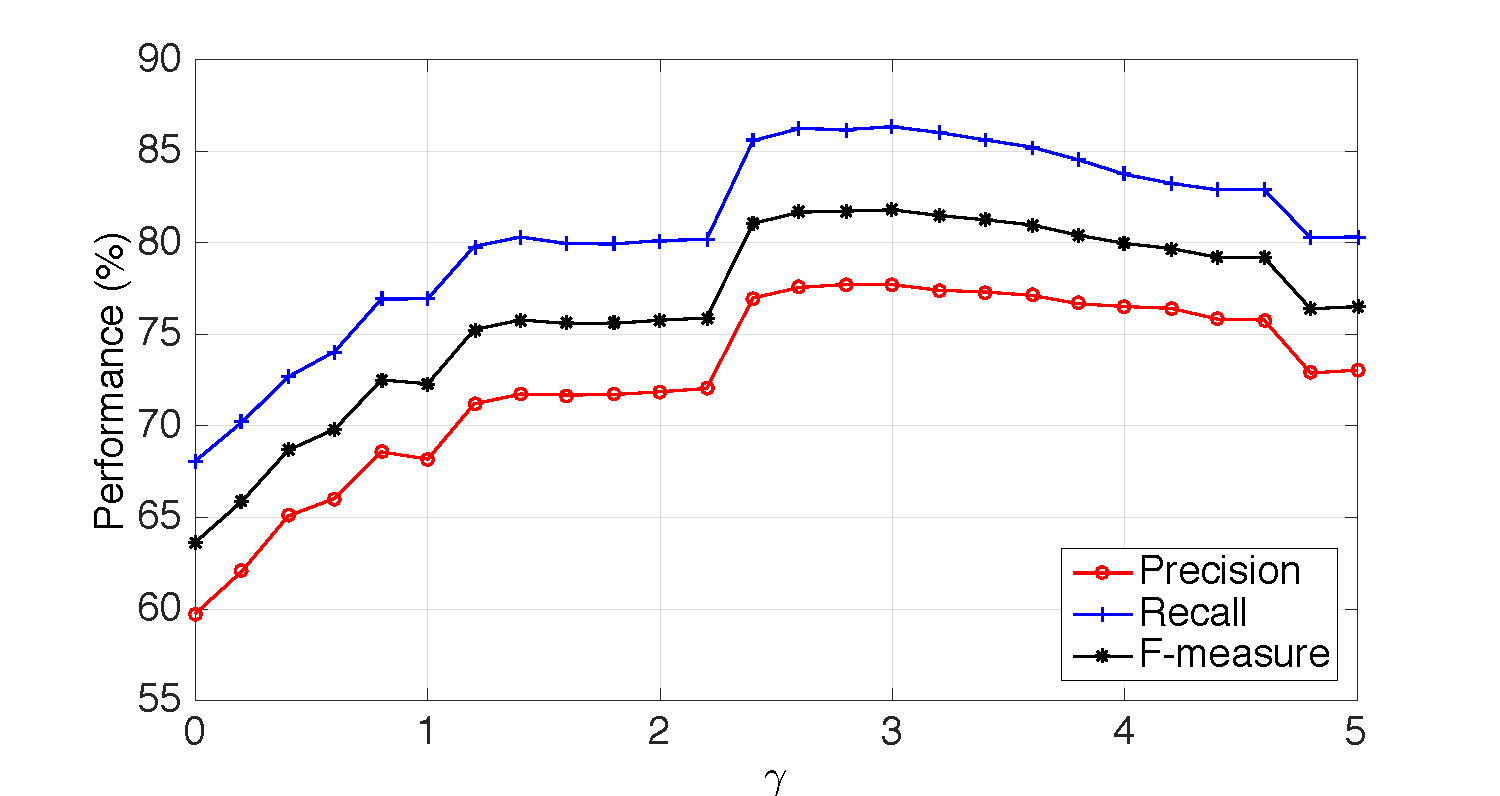
\includegraphics[width=.8\textwidth]{./chapters/chapter3/images/PROBAvsTHR.pdf} 
\caption{Effect of threshold $\gamma$ on the performance of state transition probability based algorithm simulated with Athemium dataset.}
\label{fig:L6} 
\end{figure}

Although the additional subroutines significantly improve the performance of LAE based algorithm with Athemium data, it is still less effective when applied to other dataset with more confusions among combinations as well as too much \emph{ghost power} consumed by unmonitored devices such as REDD \emph{House 1}~\cite{Kolter11redd}, as illustrated in Figure~\ref{fig:L7}. In this dataset, besides the devices connected to an individual power meter, the total power consumption of other unmonitored devices can be considered as consumed by a unique unknown device. Though there are over 20 channels, we use only nine channels as shown in Table~\ref{table:t3}, because the others have no activation of devices. Besides, two main phases of electricity are combined to have a unique main power signal.
As shown in Figure~\ref{fig:L7}, the precision of $l1$-norm minimization based algorithm can be improved from 58.63$\%$ to 60.75$\%$ and the recall from 64.62$\%$ to 70.43$\%$ with state transition probability. Nevertheless, they are still lower than the performance given by the edge detection one, with $pr=80.95\%$ and $rc = 70.58\%$, respectively. Therefore, in the next chapter, a new monitoring system will be used to significantly improve the performance of NILM algorithms based on probability information of each device provided by an additional sensor network.

\begin{table}
\caption{Power demand of devices in REDD dataset \emph{House 1}.}\label{table:t3}
\begin{center}
\begin{tabular}{|c|c|c|c|}
\hline
Power demand (watt)& State 1&State 2&State 3 \\ \hhline{|=|=|=|=|}
Oven&4140&4075&3377 \\ \hline
Fridge &193&423 & \\ \hline
Dish washer & 214& 1107 & \\ \hline
Lighting & 169 & 275 & 345 \\ \hline
Microwave &1531 & 1571 & 1396 \\ \hline
gfi bathroom & 1595 & & \\ \hline
Outlet & 1056 & & \\ \hline
Outlet & 1521 & & \\ \hline
Washer dryer & 5097 & 5250 & 5008 \\ \hline
\end{tabular}
\end{center}
\end{table}

\begin{figure}
\centering
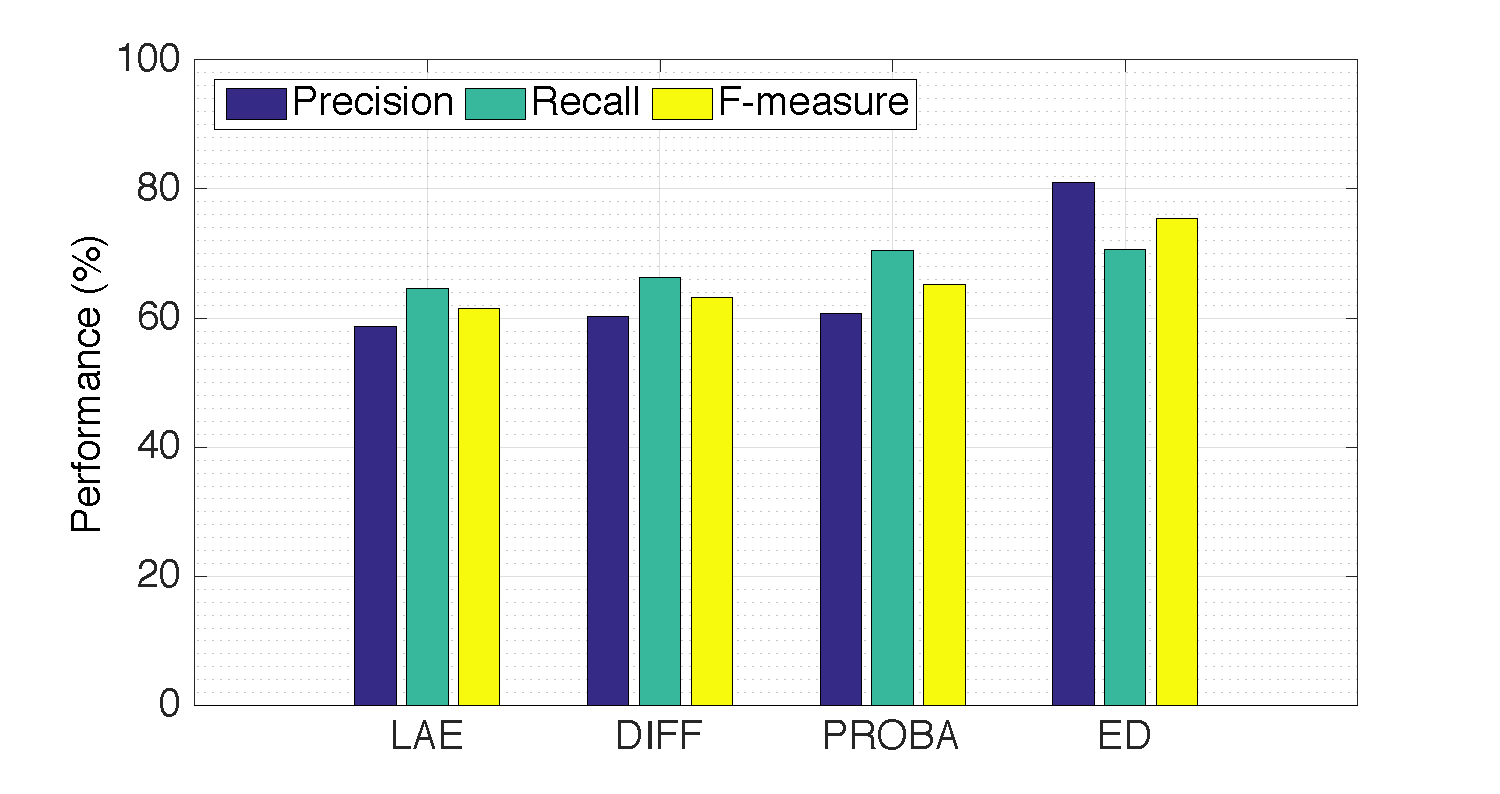
\includegraphics[width=.8\textwidth]{./chapters/chapter3/images/R1_l1_perf.pdf} 
\caption{Performance of the proposed algorithms including LAE, state difference based (DIFF) and transition probability based (PROBA) compared with the edge detection (ED) algorithm applied to REDD \emph{House 1}.}
\label{fig:L7} 
\end{figure}

